\documentclass[a0paper,25pt,ngerman]{tikzposter} % See Section 3
\title{\bfseries Warp-Drives im 23. Jahrhundert} \institute{Inst} % See Section 4.1
\author{\bfseries Zefran Cochrane} 
\institute{DLR - Deutsches Zentrum für Luft- und Raumfahrt}

\titlegraphic{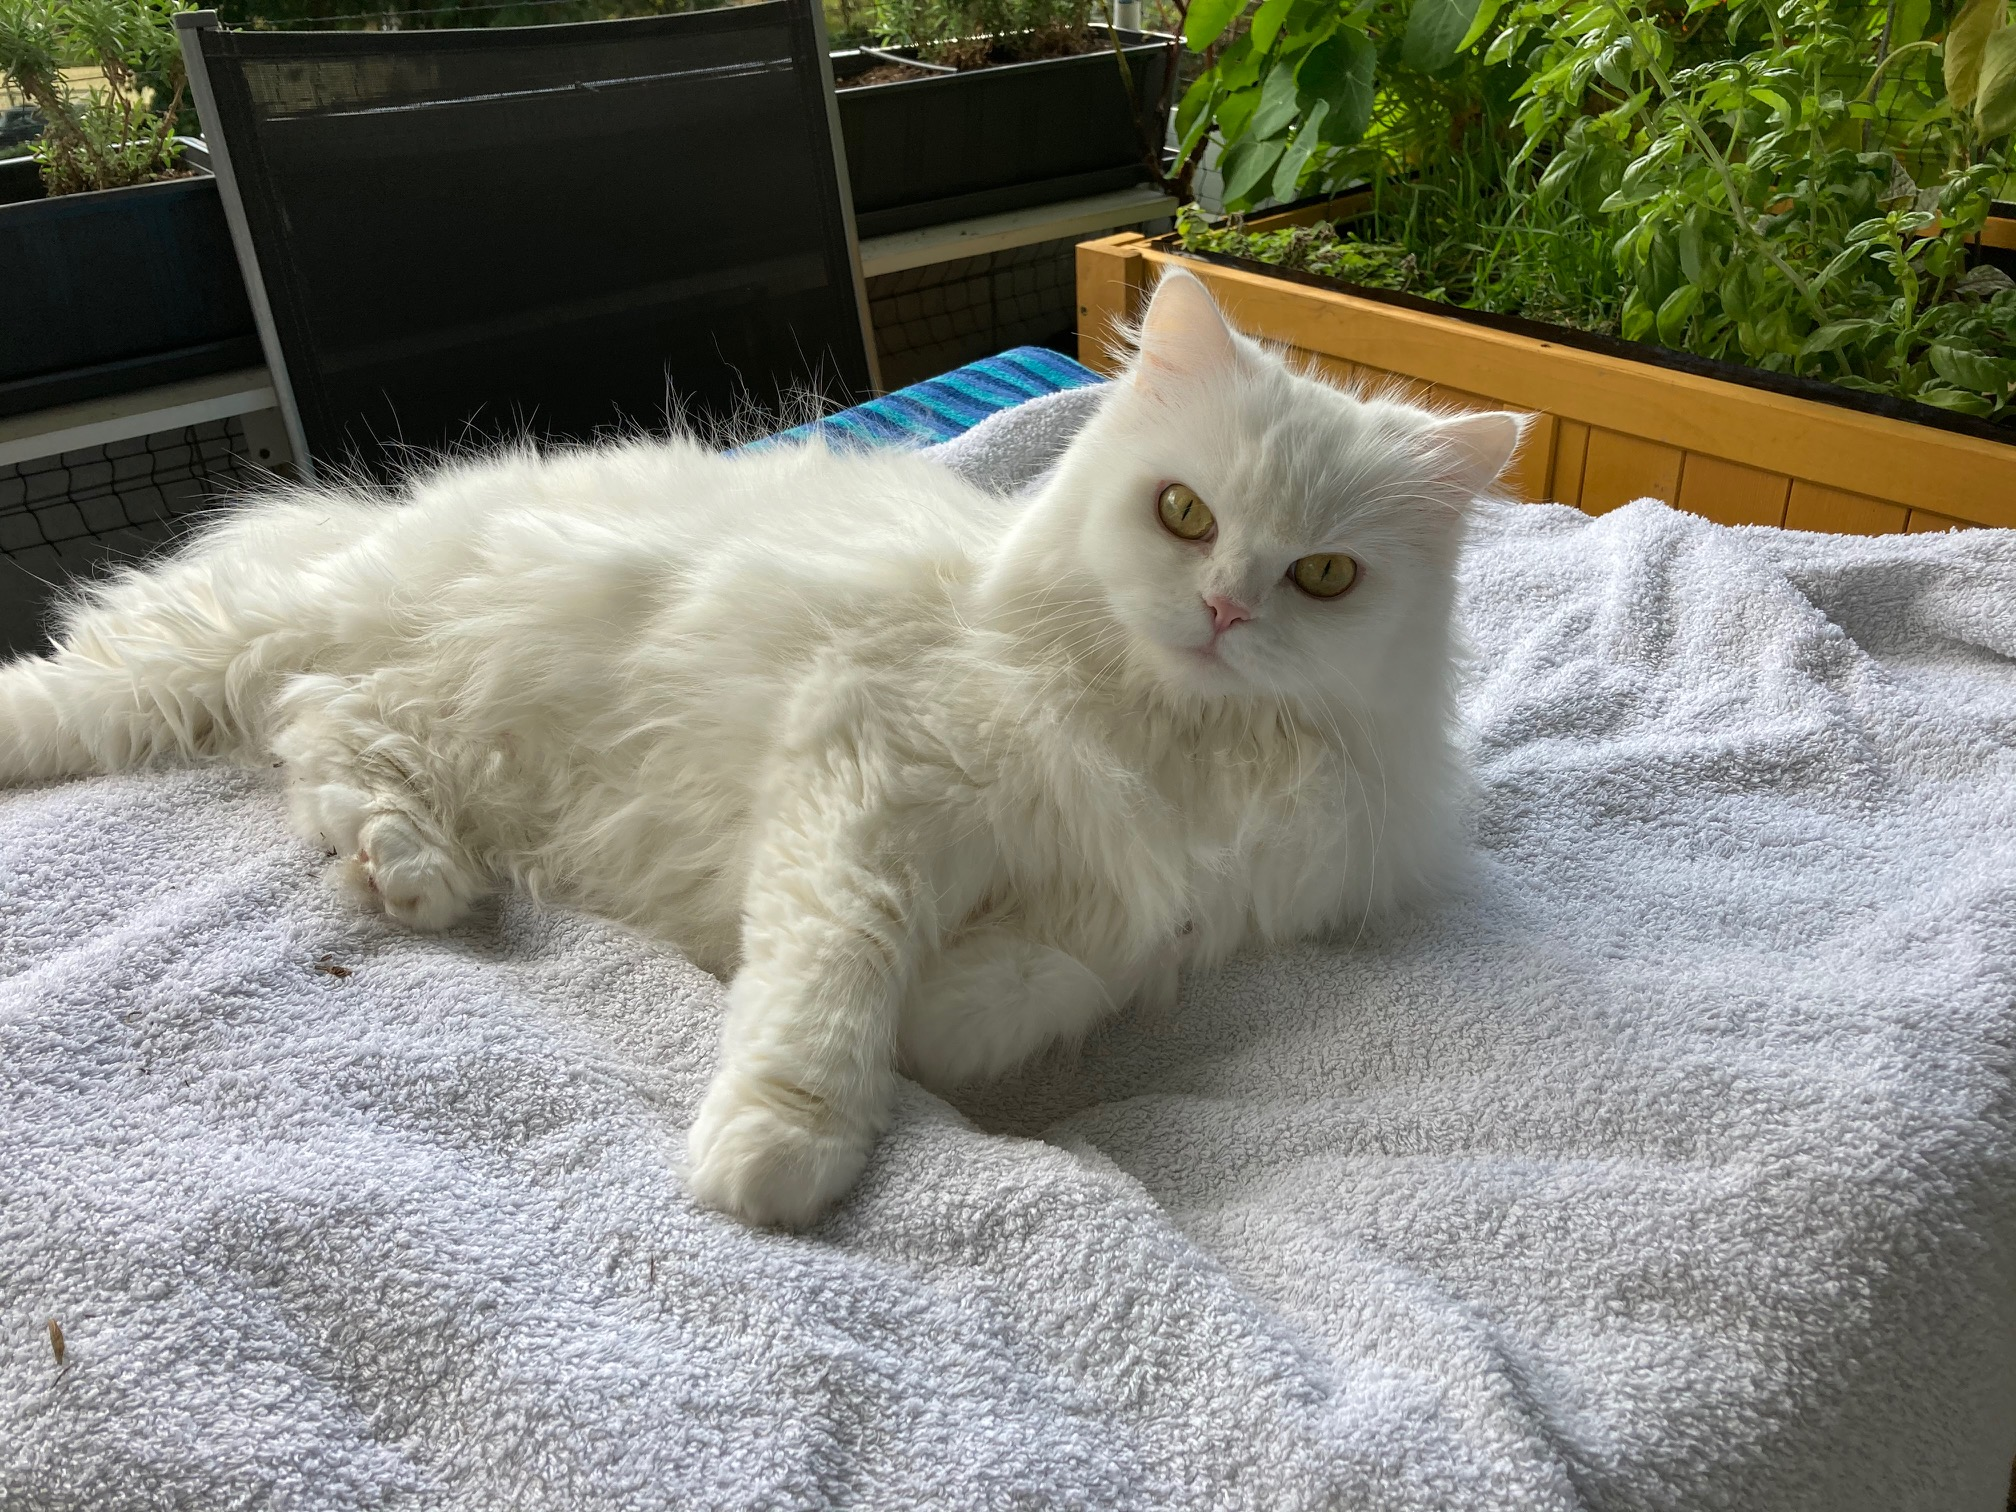
\includegraphics[width=4cm]{./Bilder/Katze1}}
\usetheme{Board} % See Section 5

%\usecolorstyle[colorPalette=BlueGrayOrange]{Britain}
%    \usebackgroundstyle{Rays}
%    \usetitlestyle{Default}
%    \useblockstyle{Default}
%    \useinnerblockstyle{Default}
%    \usenotestyle{Corner}

\usepackage{babel}
\usepackage{blindtext}
\usepackage[]{eso-pic}

%Default, Rays, Basic,Simple, Envelope, Wave, Board, Autumn, and Desert.

\begin{document}

\maketitle % See Section 4.1

\begin{columns} % See Section 4.4
\column{0.7} % See Section 4.4
\block{Grundlagen}{
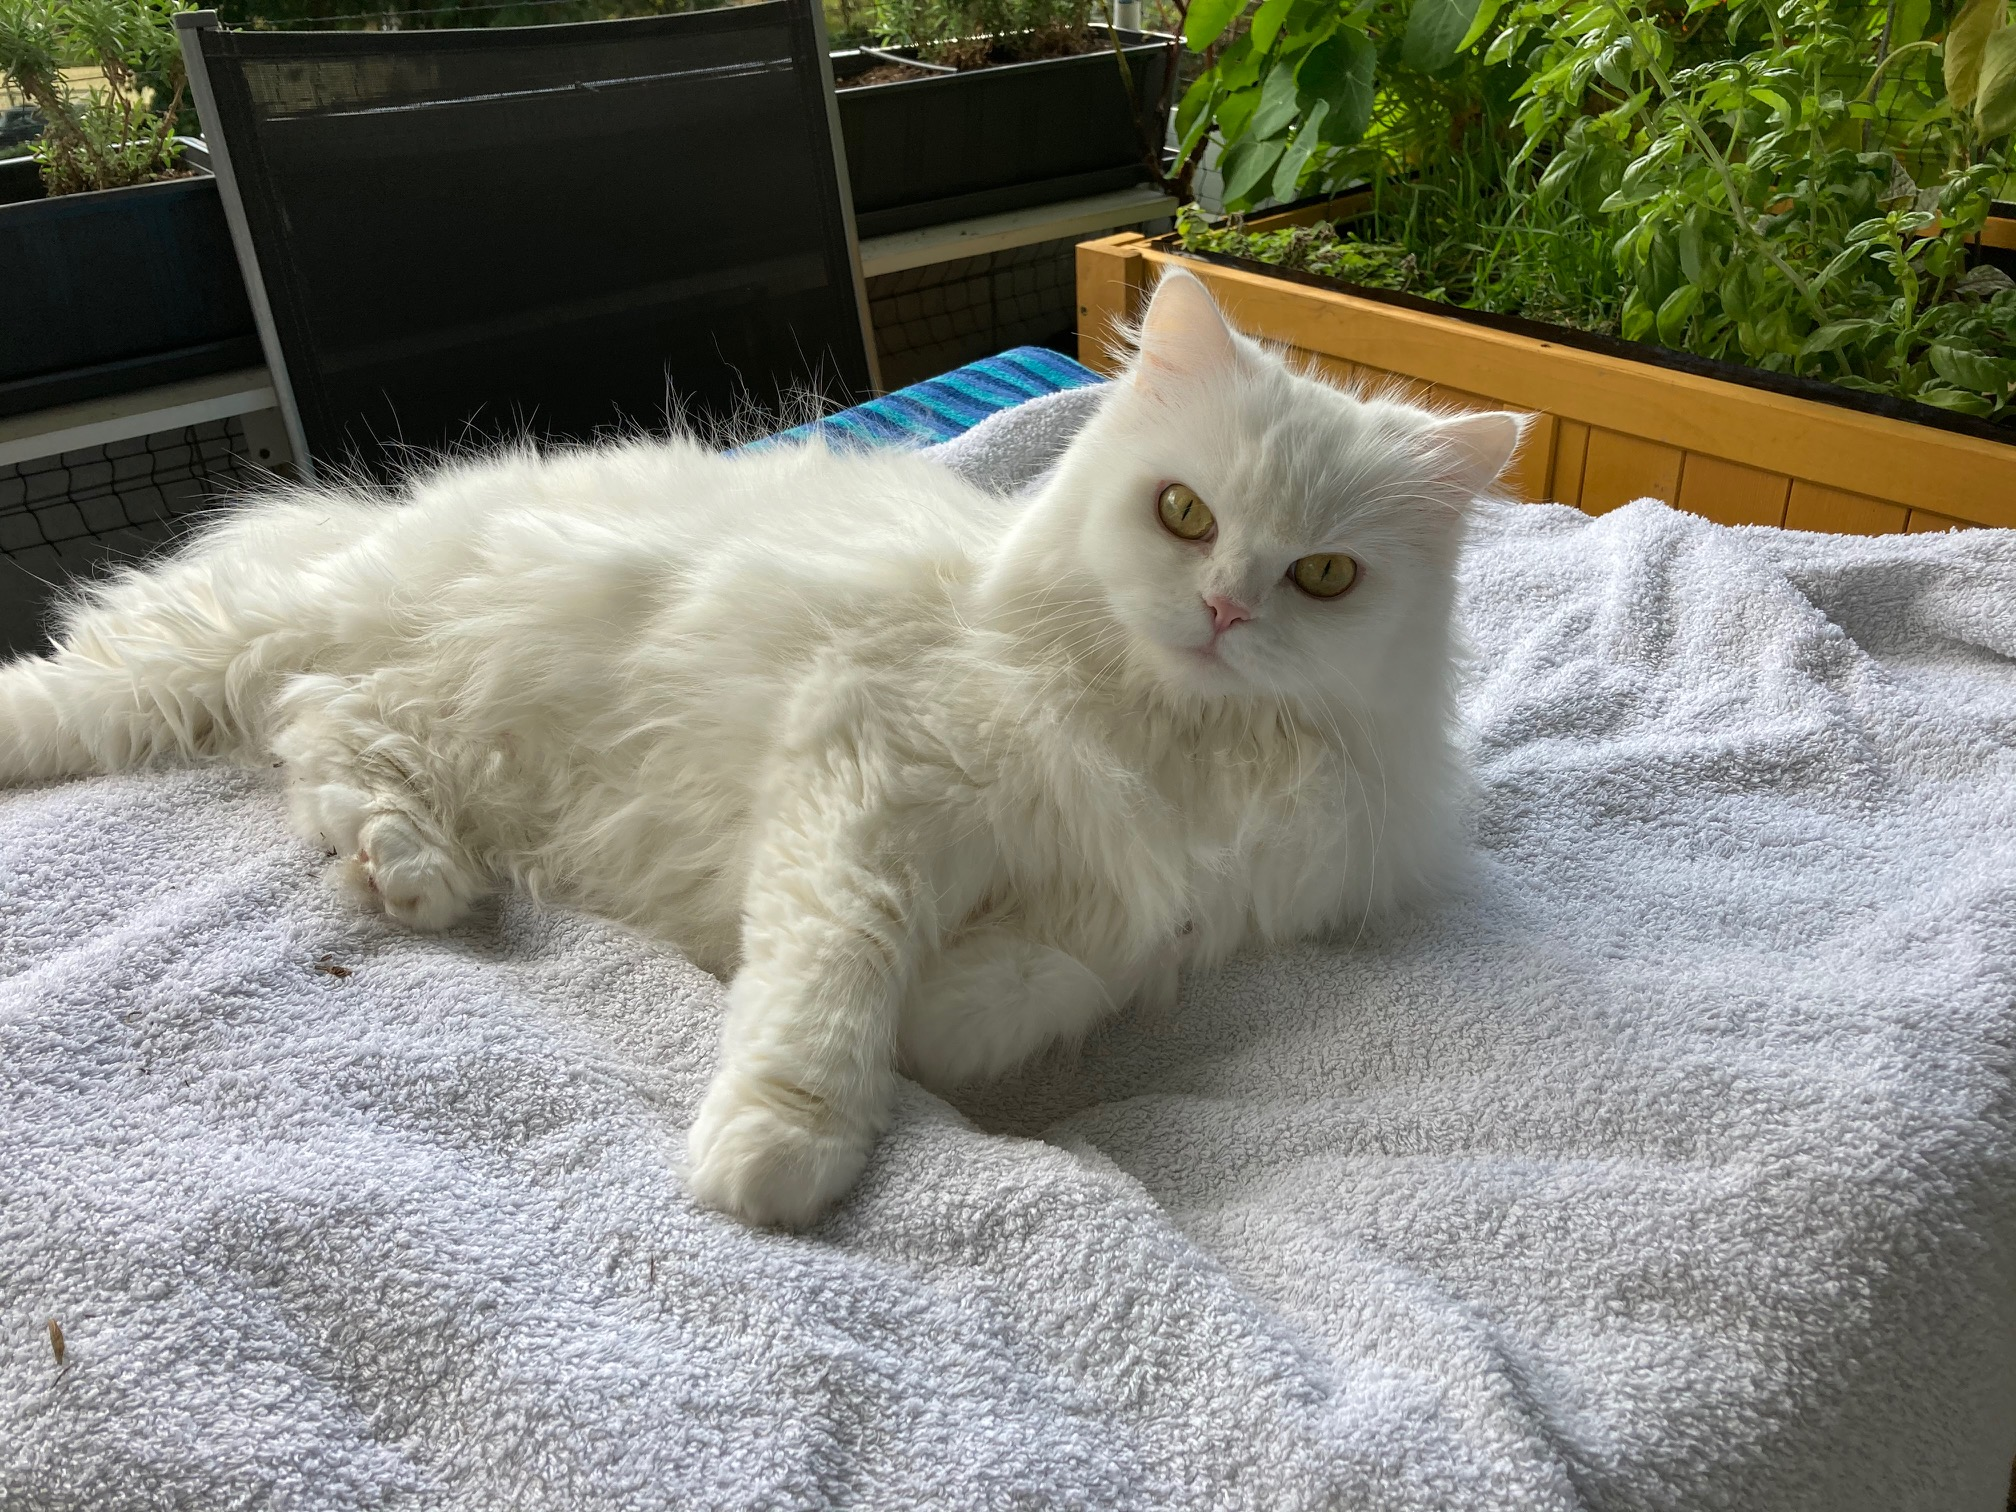
\includegraphics[width=\linewidth]{./Bilder/Katze1}
}
\note[width=20cm,targetoffsetx=-25cm, targetoffsety=-10cm,roundedcorners=30]{\blindtext}
\column{0.3}
\block{BlocktitleC}{
\blindtext[2] 
}
\end{columns}

\begin{columns} % See Section 4.4
\column{0.3} % See Section 4.4
\block{BlocktitleB}{Blocktext}
\column{0.7}
\block{BlocktitleC}{Blocktext}
 % See Section 4.3
\end{columns}

\begin{columns} % See Section 4.4
\column{0.5} % See Section 4.4
\block{~}{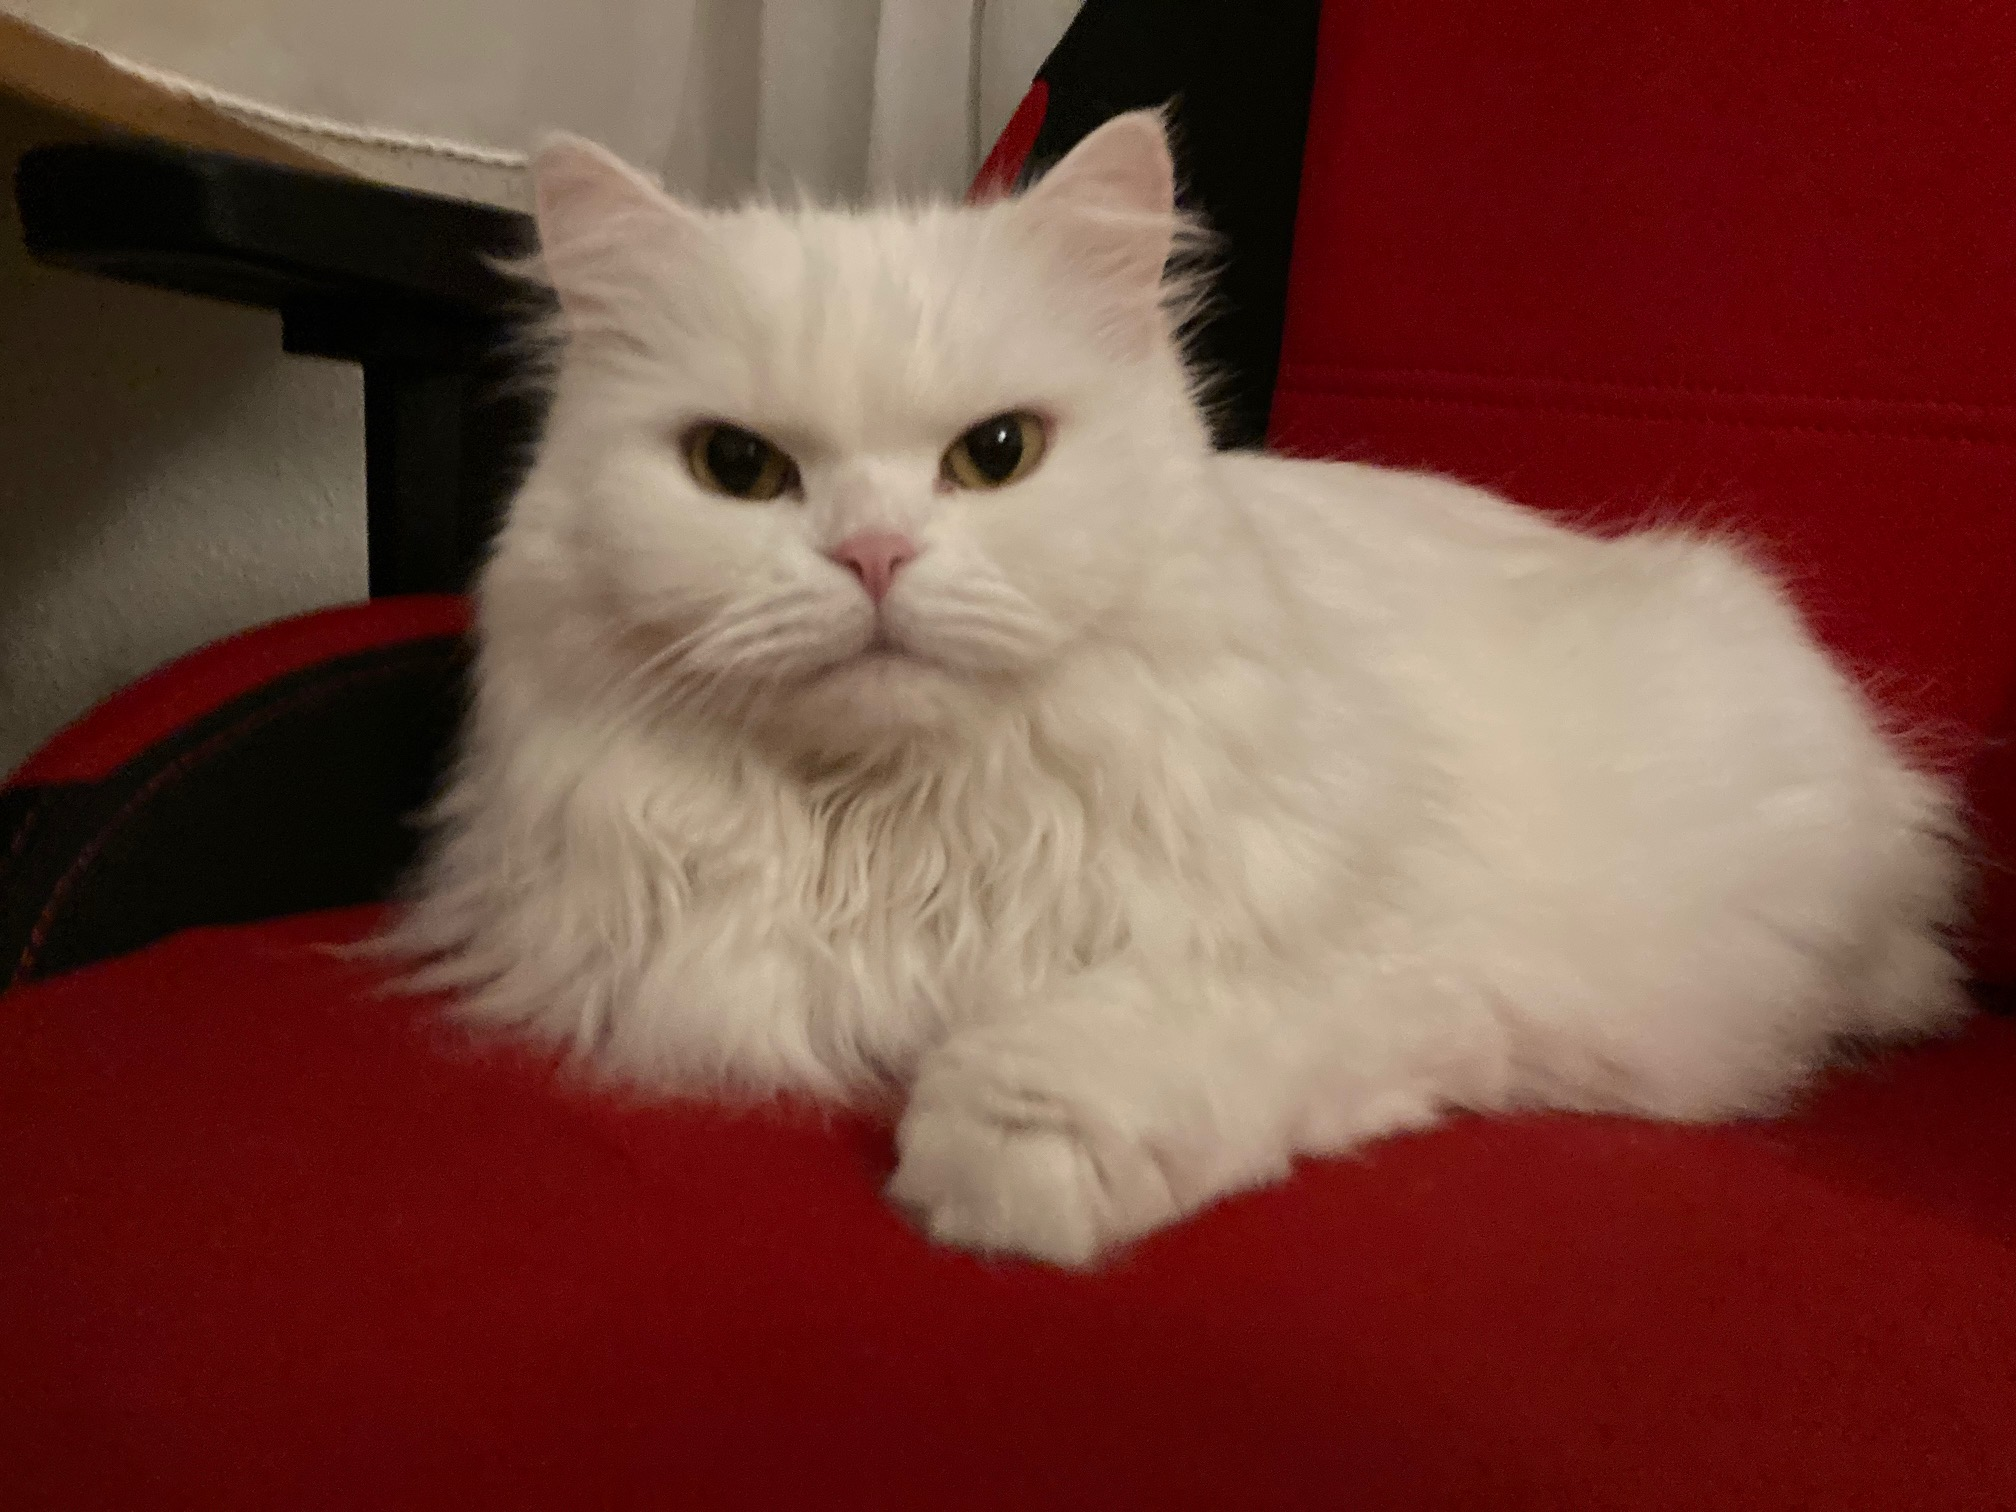
\includegraphics[width=\linewidth]{./Bilder/Katze2}}
\end{columns}

\begin{columns} % See Section 4.4
\column{0.5} % See Section 4.4
\block{Bibliografie}{
}
\end{columns}



\end{document}